\section{Harmonizer}
The harmonizer is responsible for finding the ``best'' harmonization, with respect to the weights of each progression defined in the harmonic style, for a given melody. It is defined in the Harmonization class and treats all possible sequences of chord progressions and their weights as a shortest path graph problem. Therefore it makes use of the NetworkX library,\footnote{https://networkx.github.io} a popular python library providing classes and algorithms for working with networks and graphs. 

The algorithm of the harmonizer can be summarized by the following steps:
\begin{enumerate}
  \item Find all potential progressions
  \item Build a graph from these progressions
  \item Find the shortest path in the graph
  \item Build a list of progressions from the shortest path
\end{enumerate}
These steps are depicted further in the following paragraphs, figure \ref{fig:4} shows the harmonization process of the melody ``0, 0, 0'' with the harmonic style defined in ``dummy\_style.json''.

\subsection{Finding Potential Progressions}
The harmonization algorithm starts with an harmonic style (as defined above) and a melody as input. Furthermore, the keynote and octave are given by the user in order to ``ground'' the output of final harmonization to specific notes instead of relative intervals. The maximum weight of all potential progressions is saved in order to normalize all weights later on, in order to find the shortest path (i.e. smallest sum of weights) instead of the longest.

For each note in the melody, all progressions in the harmonic style are iterated and each progression is checked whether it is a potential harmonization for the considered note. This is the case if the length of the progression is shorter than the length of the melody after the considered note (i.e. the progression is not longer than the remaining melody) and the considered and following notes are included in the respective chords of the progression. If this holds true, the progression is saved as a potential harmonization for the considered and the following notes.

\subsection{Building the Graph}
From these potential progressions, a directed weighted graph is built to be able to perform a path search with established graph search algorithms. First of all, a ``START'' node is added to the empty graph. For each potential progression for the first note of the melody, a node is created annotated with the first chord of the progression and a ``1'' indicating the current position. The position is attached to the node to account for progressions of different lengths. This set of nodes is then connected to the starting node. (Fig. \ref{fig:41})

Additionally, a node is created for every last chord of the progressions, again annotated with the chord and position (depending on the length of the progression). An edge is added between two nodes if the transition is possible, indicating the chord progression itself and the weight taken from the harmonic style. (Fig. \ref{fig:42}) All weights are calculated by subtracting the actual weight from the maximum weight, therefore the largest weight gets weight 0 and we have to solve a shortest / cheapest path problem, for which more algorithms exist. If more than one transition between two nodes is possible, only the progression with the largest weight is considered since all others can not be part of the best path.

This procedure is repeated until the nodes for the potential harmonization of the last note of the melody are created. These are then connected to the ``END'' node, and a path can be searched for between ``START'' and ``END'' node. (Fig. \ref{fig:43})


\subsection{Shortest Path}
As described above, the progressions with the largest weights in the style definition (= most desirable progressions) possess the smalles weights in the graph. Therefore the algorithm has to find the shortest path (weights are seen as distances) between the ``START'' and ``END'' nodes. We decided on the Dijkstra algorithm for this matter, since we are looking for a single source path in a graph with non-negative weights. To speed up computation for long melodies or extensive harmonic styles, we used a bidirectional implementation. The path found by this algorithm in the example graph can be seen in Fig. \ref{fig:44}.

% bidirectional dijkstra https://en.wikipedia.org/wiki/Dijkstra's_algorithm https://en.wikipedia.org/wiki/Bidirectional_search
% figure of dijkstra
% optimization problem

\subsection{Final Harmonization}
In the final step, the algorithm creates the list of chords representing the final harmonization. This is achieved by iterating the nodes of the shortest path from starting to final node, appending the chords attached to the edges connecting the nodes. This list of chords is then returned to the calling function and can further be worked with.

\begin{figure}[!tbp]
\vspace*{-3cm}
\centering
\begin{subfigure}[b]{0.43\linewidth}
   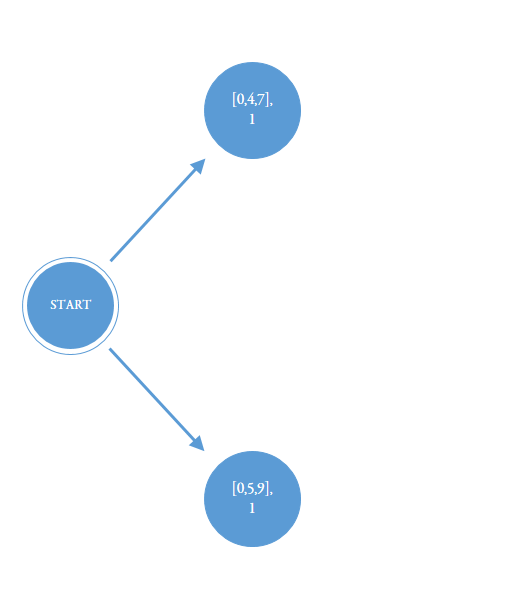
\includegraphics[width=\linewidth]{Chapters/pic/41}
   \caption{Adding START node and first chords of first progression}
   \label{fig:41} 
\end{subfigure}
\hfill
\begin{subfigure}[b]{0.49\linewidth}
   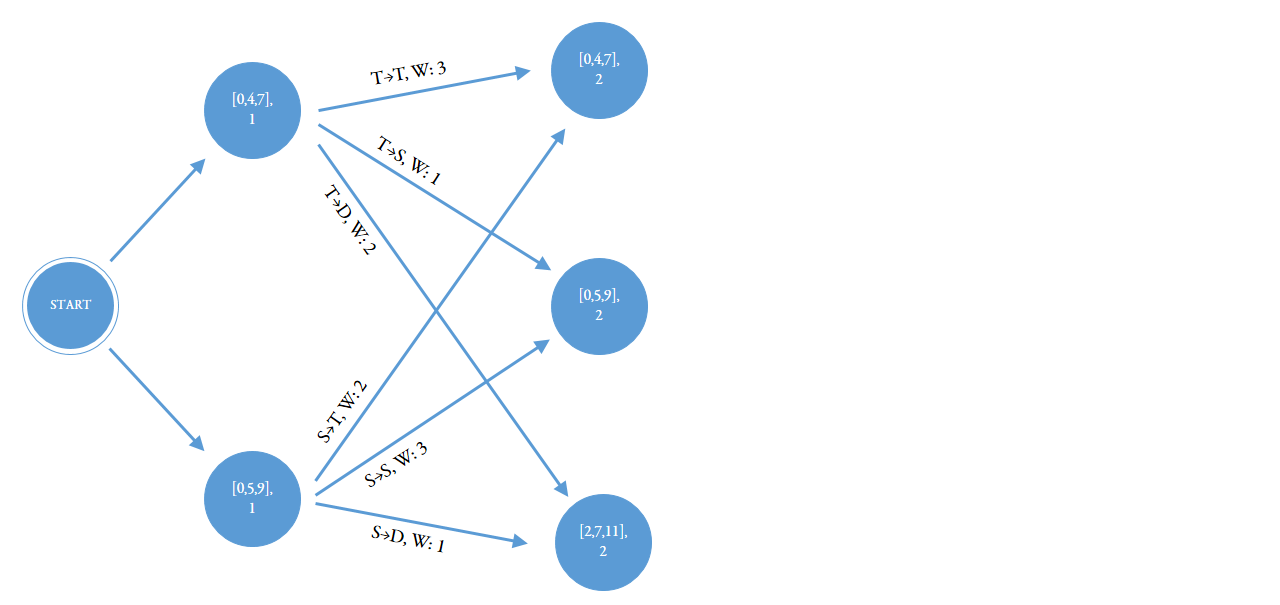
\includegraphics[width=\linewidth]{Chapters/pic/42}
   \caption{Adding last chords of first progression}
   \label{fig:42}
\end{subfigure}

\begin{subfigure}[b]{1.2\linewidth}
   \hspace{-1.1cm}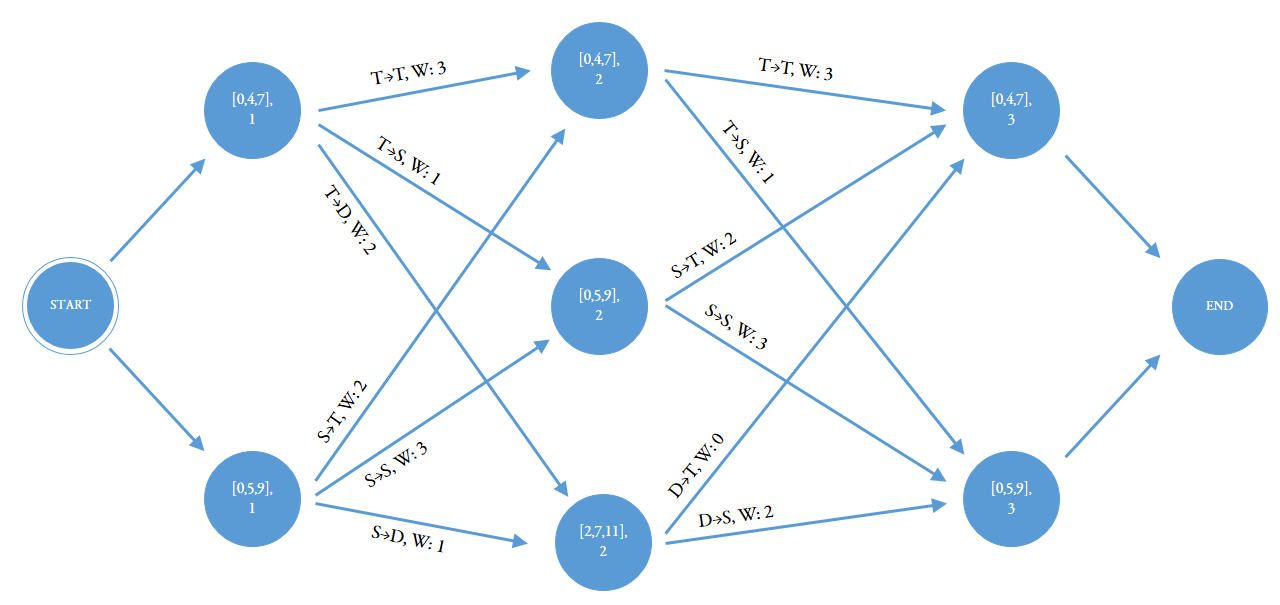
\includegraphics[width=\linewidth]{Chapters/pic/43}
   \hspace{-1.1cm}\caption{Completed graph for melody ``0, 0, 0''}
   \label{fig:43}
\end{subfigure}

\begin{subfigure}[b]{1.2\linewidth}
   \hspace{-1.1cm}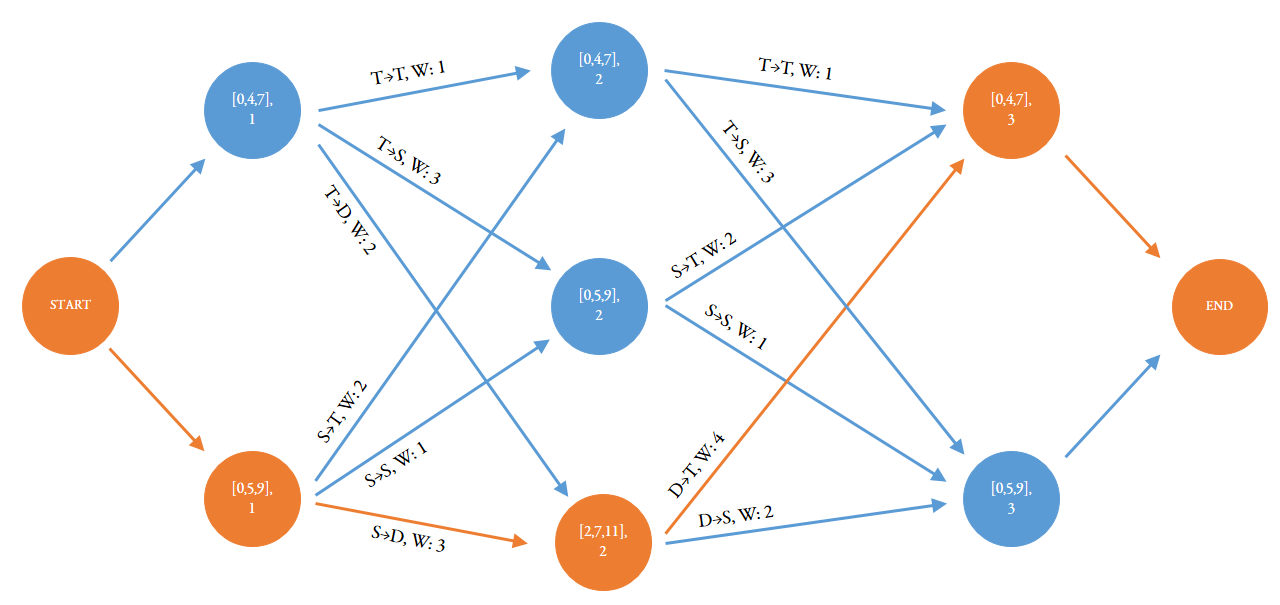
\includegraphics[width=\linewidth]{Chapters/pic/44}
   \hspace{-1.1cm}\caption{Shortest path found by bidirectional Dijkstra}
   \label{fig:44}
\end{subfigure}

\caption{Selected steps of the harmonization with ``dummy\_style.json''}
\label{fig:4}
\end{figure}

